% Section content template for individual Educative lessons
% This file contains the actual content for a specific section
% Generated from Educative API section content

% Section: The Reality Is More Complicated
% Section ID: 5471711817891840
% Section Slug: the-reality-is-more-complicated
% Generated: 2025-12-07T22:38:43.056927

\subsection{Introduction}\label{n3S6U8v7EPnC_WNy-A6tX}
\\
Now that we've understood the design well, let's see how YouTube can optimize the usage of storage and network demands while maintaining good quality of experience (QoE)(QoE is the measure of a customer's satisfaction with the experience of a particular service.) for the end user.
\\
When talking about providing effective service to end users, the following three steps are important:

\begin{itemize}
\item
\protect\phantomsection\label{YHAskX-YYEWfEEOMSd4ri}
\textbf{Encode}: The raw videos uploaded to YouTube have significant storage requirements. It's possible to use various encoding schemes to reduce the size of these raw video files. Apart from compression, the choice of encoding scheme will also depend on the types of end devices used to stream the video content. Since multiple devices could be used to stream the same video, we may have to encode the same video using different encoding schemes resulting in one raw video file being converted into multiple files each encoded differently. This strategy will result in a good user-perceived experience because of two reasons: users will save bandwidth because the video file will be encoded and compressed to some limit, and the encoded video file will be appropriate for the client for a smooth playback experience.
\item
\protect\phantomsection\label{1o8jJXbMDClm3C2XNG3qd}
\textbf{Deploy}: For low latency, content must be intelligently deployed so that it is closer to a large number of end users. Not only will this reduce latency, but it will also put less burden on the networks as well as YouTube's core servers.
\item
\protect\phantomsection\label{tAZAJ0Ba23eV5qkfc5K5x}
\textbf{Deliver}: Delivering to the client requires knowledge about the client or device used for playing the video. This knowledge will help in adapting to the client and network conditions. Therefore, we'll enable ourselves to serve content efficiently.
\end{itemize}
\\
Let's understand each phase in detail now.

\subsection{Encode}\label{pzQsJuTOfVh9st3883n67}
\\
Until now, we've considered encoding one video with different encoding schemes. However, if we encode videos on a per-shot basis, we'll divide the video into smaller time frames and encode them individually. We can divide videos into shorter time frames and refer to them as segments. Each segment will be encoded using multiple encoding schemes to generate different files called chunks. The choice of encoding scheme for a segment will be based on the detail within the segment to get optimized quality with lesser storage requirements. Eventually , each shot will be encoded into multiple chunk sizes depending on the segment's content and encoding scheme used. As we divide the raw video into segments, we'll see its advantages during the deployment and delivery phase.
\\
Let's understand how the per-segment encoding will work. For any video with dynamic colors and high depth, we'll encode it differently from a video with fewer colors. This means that a not-so-dynamic segment will be encoded such that it's compressed more to save additional storage space. Eventually , we'll have to transfer smaller file sizes and save bandwidth during the deployment and streaming phases.

\begin{figure}[htbp]
 \centering
 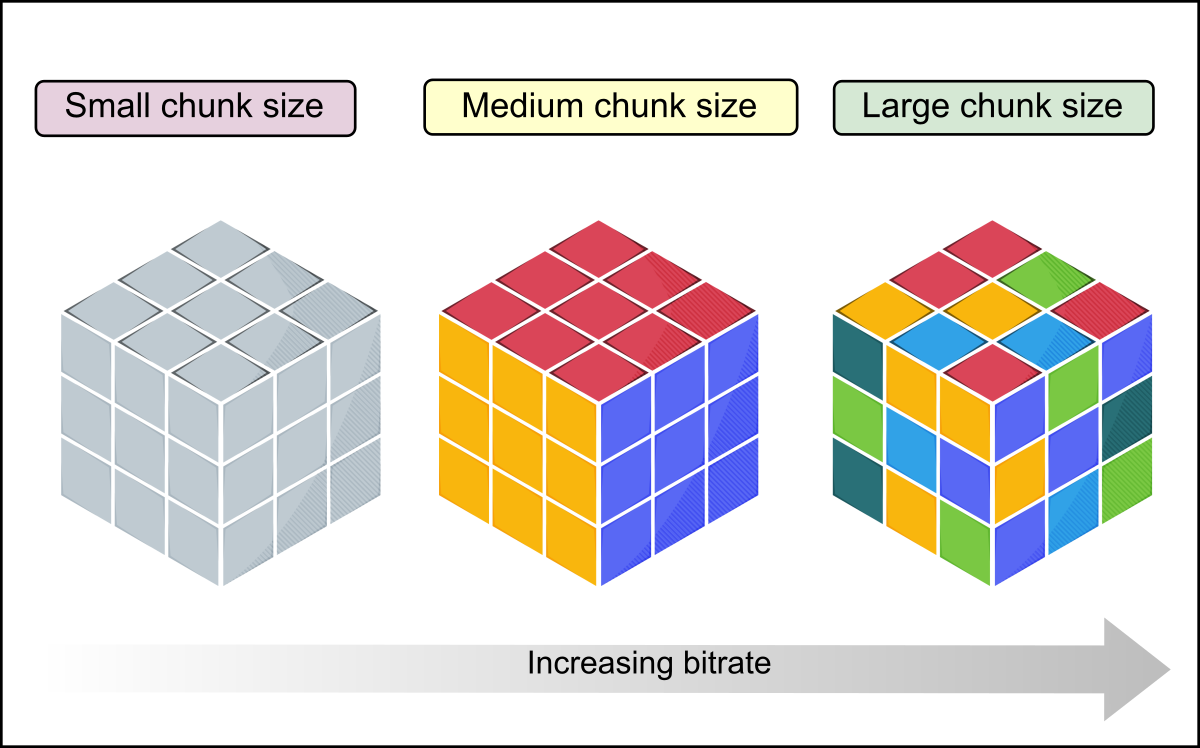
\includegraphics[width=0.5\textwidth]{Images/chapter_26/section_5471711817891840/6132756205928448.png}
 \caption{Higher quality requiring higher bitrate from left to right}
\end{figure}

Using the strategy above, we'll have to encode individual shots of a video in various formats. However, the alternative to this would be storing an entire video (using no segmenting) after encoding it in various formats. If we encode on a per-shot basis, we would be able to optimally reduce the size of the entire video by doing the encoding on a granular level. We can also encode audio in various formats to optimally allow streaming for various clients like TVs, mobile phones, and desktop machines. Specifically , for services like Netflix, audio encoding is more useful because audios are offered in various languages.

\begin{figure}[htbp]
 \centering
 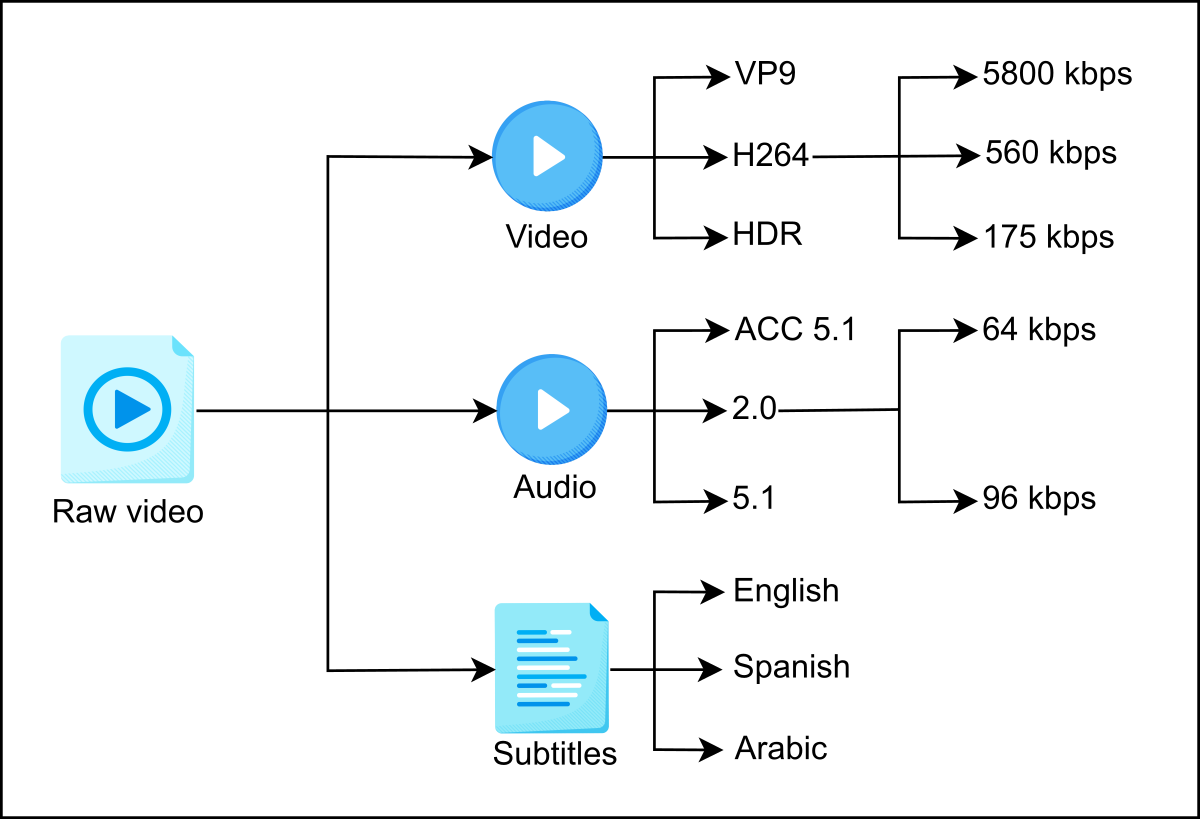
\includegraphics[width=0.5\textwidth]{Images/chapter_26/section_5471711817891840/5397229399834624.png}
 \caption{A raw video file being encoded into different formats including its audio and subtitles}
\end{figure}

\subsection{Deploy}\label{7qcrzMEH3NyueFnADxkfE}
\\
As discussed in our design and evaluation sections, we have to bring the content closer to the user. This has three main advantages:

\begin{enumerate}
\item
\protect\phantomsection\label{whxaMRhpodaz9RFhcip3N}
Users will be able to stream videos quickly.
\item
\protect\phantomsection\label{lNhI3aW0ZEWGkSuUA5ucD}
There will be a reduced burden on the origin servers(The servers responsible for listening and responding to clients' requests).
\item
\protect\phantomsection\label{tNFeeKRbQQl9YRSj0IcdG}
Internet service providers (ISPs) will have spare bandwidth.
\end{enumerate}
\\
So, instead of streaming from our data centers directly, we can deploy chunks of popular videos in CDNs and point of presence (PoPs)(PoP is a point where two or more large networks combine to enable communication between their clients) of ISPs. In places where there is no collaboration possible with the ISPs, our content can be placed in internet exchange point (IXPs). We can put content in IXPs that will not only be closer to users, but can also be helpful in filling the cache of ISP PoPs.

\begin{figure}[htbp]
 \centering
 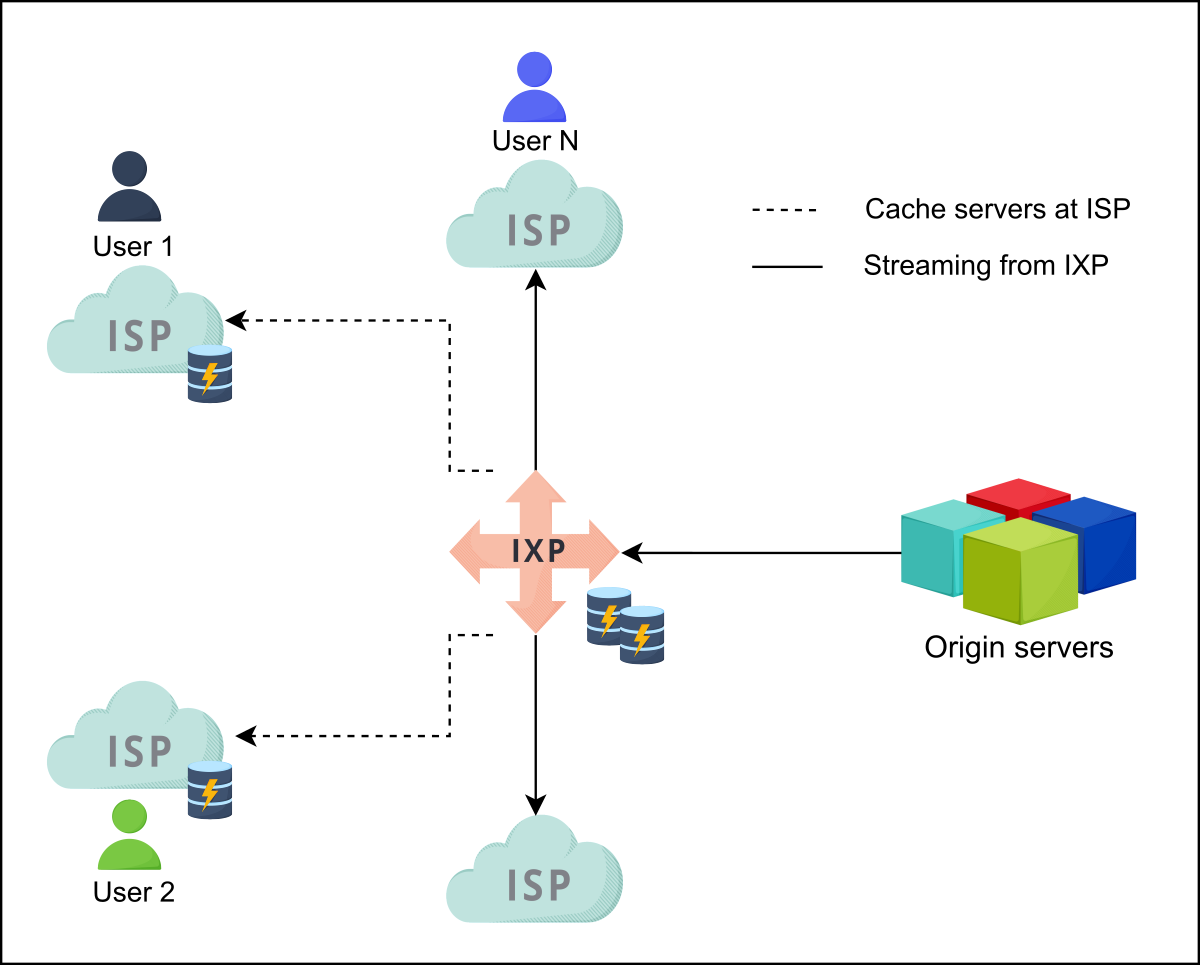
\includegraphics[width=0.5\textwidth]{Images/chapter_26/section_5471711817891840/6278092228526080.png}
 \caption{Streaming from data center to users through IXP and ISPs}
\end{figure}

We should keep in mind that the caching at the ISP or IXP is performed only for the popular content or moderately popular content because of limited storage capacity. Since our per-shot encoding scheme saves storage space, we'll be able to serve out more content using the cache infrastructure closer to end users.
\\
Additionally, we can have two types of storage at the origin servers:

\begin{enumerate}
\item
\protect\phantomsection\label{nCepWKxfzjJYe_jMVVr40}
\textbf{Flash servers}: These servers hold popular and moderately popular content. They are optimized for low-latency delivery.
\item
\protect\phantomsection\label{F6WitnTwlYenFtHSbsQXI}
\textbf{Storage servers}: This type holds a large portion of videos that are not popular. These servers are optimized to hold large storage.
\end{enumerate}
\begin{quote}
\textbf{Note:} When we transfer streaming content, it can result in the congestion of networks. That is why we have to transfer the content to ISPs in off-peak hours.
\end{quote}
\subsubsection{Recommendations}\label{PbjovK0HXtT_2AQVF2XTk}
\\
YouTube recommends videos to users based on their profile, taking into account factors such as their interests, view and search history, subscribed channels, related topics to already viewed content, and activities on content such as comments and likes.
\\
An approximation of the recommendation engine of YouTube is provided below. YouTube filters videos in two phases:

\begin{enumerate}
\item
\protect\phantomsection\label{y3mVFJEfS5MIsFVKWLBY1}
\textbf{Candidate generation}: During this phase, millions of YouTube videos are filtered down to hundreds based on the user's history and current context.
\item
\protect\phantomsection\label{6PoaUArGL4XQz2DBh3zb3}
\textbf{Ranking}: The ranking phase rates videos based on their features and according to the user's interests and history. Hundreds of videos are filtered and ranked down to a few dozen videos during this phase.
\end{enumerate}
\\
YouTube employs machine learning(Covington, Paul, Jay Adams, and Emre Sargin. ``Deep neural networks for youtube recommendations.'' Proceedings of the 10th ACM conference on recommender systems. 2016.) technology in both phases to provide recommendations to users.

\begin{figure}[htbp]
 \centering
 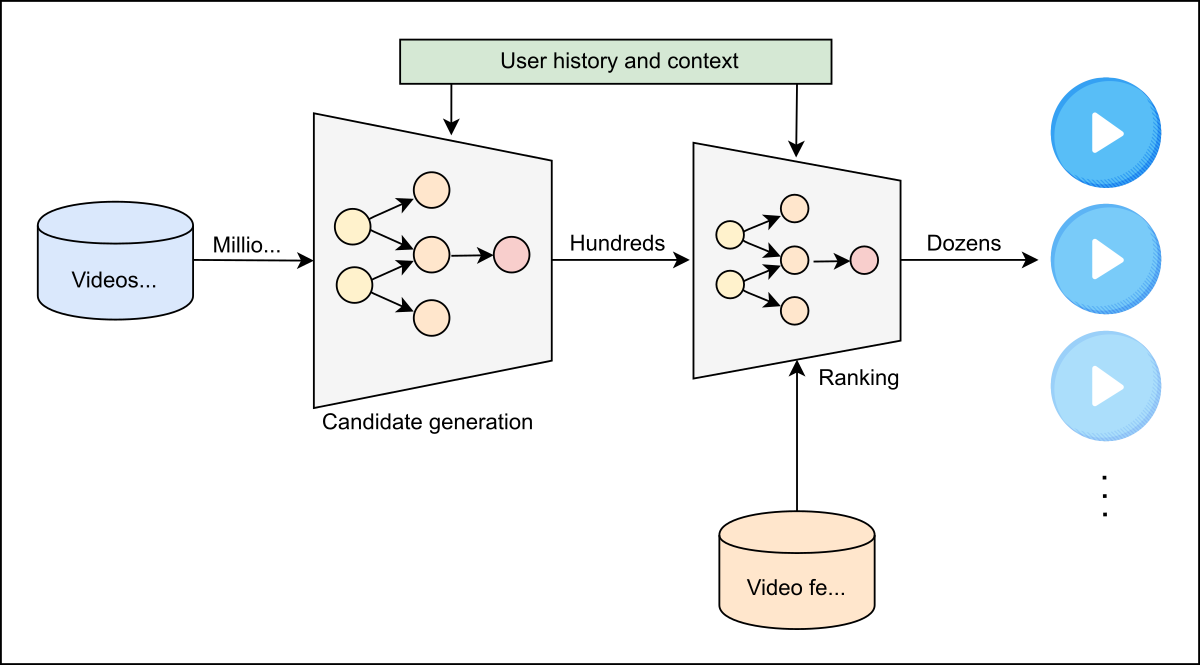
\includegraphics[width=0.5\textwidth]{Images/chapter_26/section_5471711817891840/6214101829550080.png}
 \caption{YouTube's recommendation engine using two neural networks to filter videos from millions to dozens}
\end{figure}

\begin{quote}
\textbf{Quiz:}
\textbf{Question 1:} Previously, we said that popular content is sent to ISPs, IXPs, and

CDNs. We've now discussed YouTube's feature that recommends content.

What is the difference between popular and recommended content on YouTube?
\textbf{Answer:} Recommendations are specific to users' profiles and interests, whereas popular content is recognized on a regional or global basis. It is possible to present popular content to the general audience.
\textbf{Question 2:} Can you provide some formulaic representation of how the YouTube algorithm for popular content would work?
\textbf{Answer:} To approximate a formula, we can assume a threshold value which is the weighted sum of all the considered factors like this:

$$
Th_{\text{reg}} =
Comments_{\text{wt}} \times Comments_{\text{num}}
+ Likes_{\text{wt}} \times Likes_{\text{num}}
+ Links_{\text{wt}} \times Links_{\text{num}}
+ \cdots
$$

Where:

\begin{itemize}
    \item $Th_{\text{reg}}$ is the number used to decide whether a video is viral in a specific region.
    \item $Comments_{\text{wt}}$ is the weight of the comments.
    \item $Comments_{\text{num}}$ is the number of comments.
    \item $Likes_{\text{wt}}$ is the weight of likes.
    \item $Likes_{\text{num}}$ is the number of likes.
    \item $Links_{\text{wt}}$ is the weight of the links.
    \item $Links_{\text{num}}$ is the number of links.
\end{itemize}

The cumulative sum of each weight is equal to 1.

We may also assume that different threshold levels can be considered for different regions.  
Finally, we can consider a video to be globally popular if the sum of thresholds of different regions passes a global threshold value.

YouTube may also decide to put some videos directly in the CDN depending on the channel used to upload the videos.

\textbf{Question 3:} In reference to Question 2, how often do you think that the approximation calculation for whether content is popular will be made?

On each click, like, or comment?
\textbf{Answer:} Calculation per click, like, or comment requires special infrastructure to perform calculations correctly and in real-time. This should be limited to: - The most popular channels. - Alternatively, a particular metric that triggers the computation every time it crosses a certain value. A good trigger could be an increasing number of requests made for a specific video in a shorter period of time.
\end{quote}

\subsection{Deliver}\label{Fj8yVrDADKiErPahFkAl5}
\\
Let's see how the end user gets the content on their device. Since we have the chunks of videos already deployed near users, we redirect users to the nearest available chunks. As shown below, whenever a user requests content that YouTube has recognized as popular, YouTube redirects the user to the nearest CDN.\\
\strut \\
However, in the case of non-popular content, the user is served from colocation sites or YouTube's data center where the content is stored initially. We have already learned how YouTube can reduce latency times by having distributed caches at different design layers.

\begin{figure}[htbp]
 \centering
 \begin{subfigure}[b]{0.48\textwidth}
 \centering
 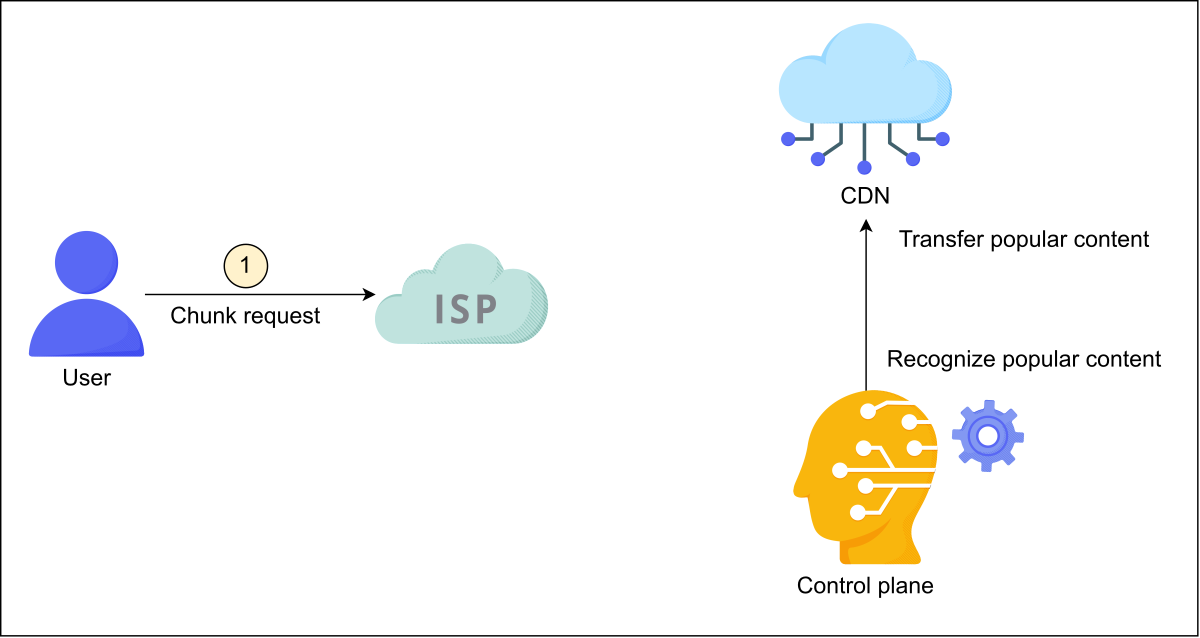
\includegraphics[width=\textwidth]{Images/chapter_26/section_5471711817891840/5499110117736448.png}
 \caption{The user requests for chunk using the ISP.}
 \end{subfigure}
 \hfill
 \begin{subfigure}[b]{0.48\textwidth}
 \centering
 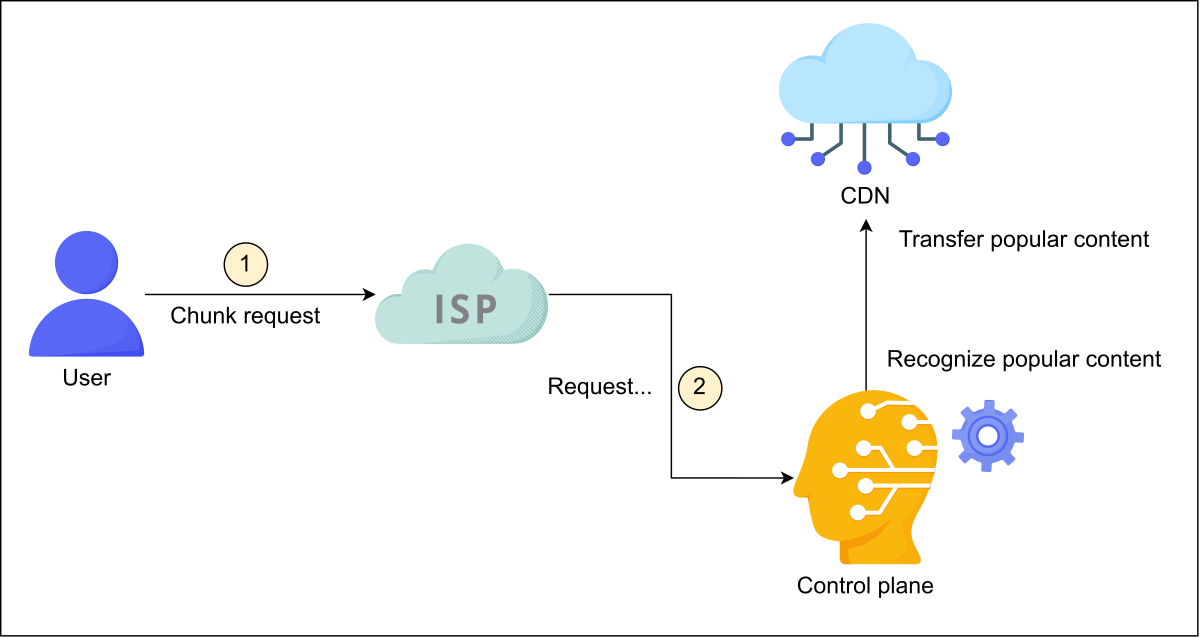
\includegraphics[width=\textwidth]{Images/chapter_26/section_5471711817891840/6138071479615488.png}
 \caption{The ISP forwards the request to the control plane of YouTube.}
 \end{subfigure}
\end{figure}

\begin{figure}[htbp]
 \centering
 \begin{subfigure}[b]{0.48\textwidth}
 \centering
 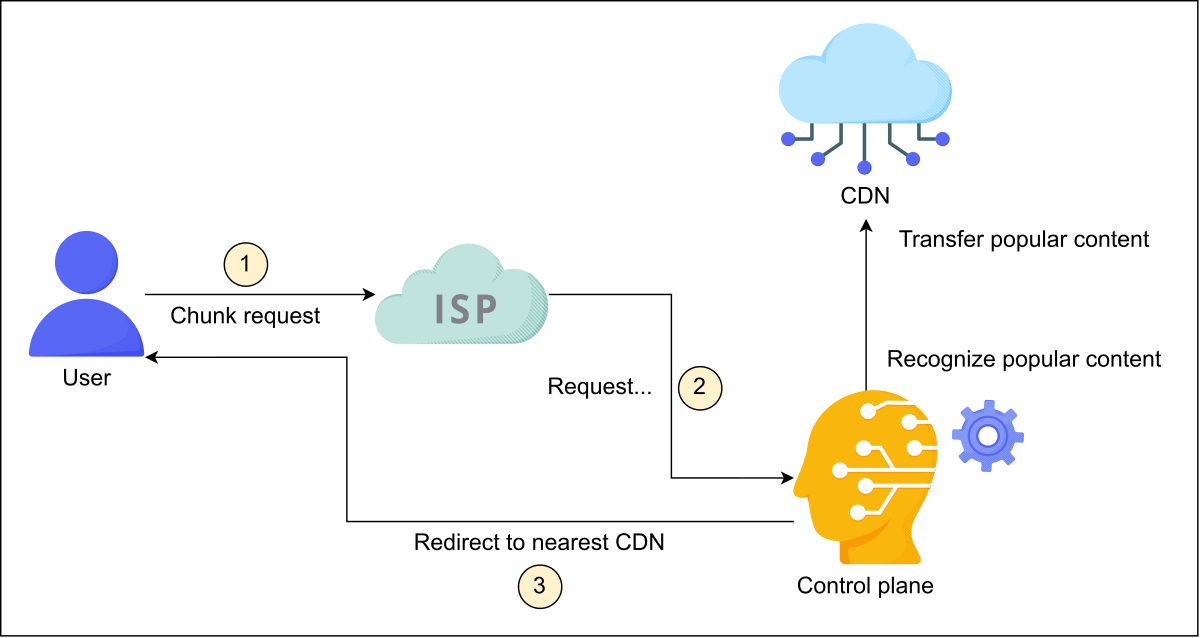
\includegraphics[width=\textwidth]{Images/chapter_26/section_5471711817891840/6120543701303296.png}
 \caption{The control plane redirects the user to the nearest CDN.}
 \end{subfigure}
 \hfill
 \begin{subfigure}[b]{0.48\textwidth}
 \centering
 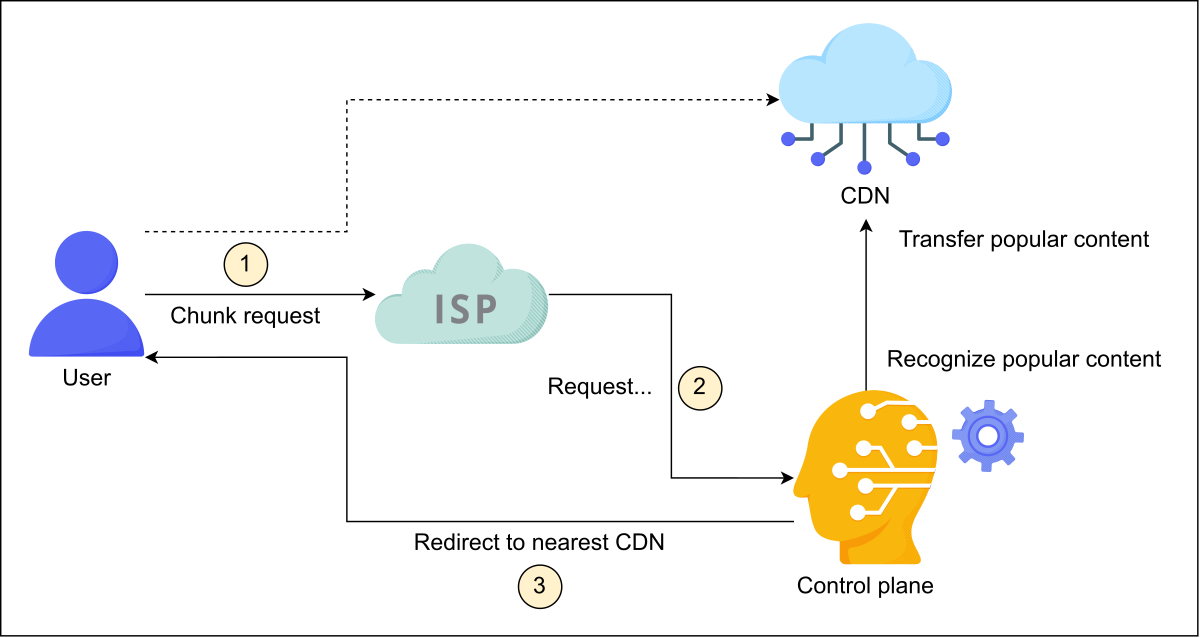
\includegraphics[width=\textwidth]{Images/chapter_26/section_5471711817891840/5867951591129088.png}
 \caption{The user starts streaming from the nearest CDN.}
 \end{subfigure}
\end{figure}

\subsubsection{Adaptive streaming}\label{PvHnuSSzfrWL8hTfd3jv3}
\\
While the content is being served, the bandwidth of the user is also being monitored at all times. Since the video is divided into chunks of different qualities, each of the same time frame, the chunks are provided to clients based on changing network conditions.\\
\strut \\
As shown below, when the bandwidth is high, a higher quality chunk is sent to the client and vice versa.\\

\begin{figure}[htbp]
 \centering
 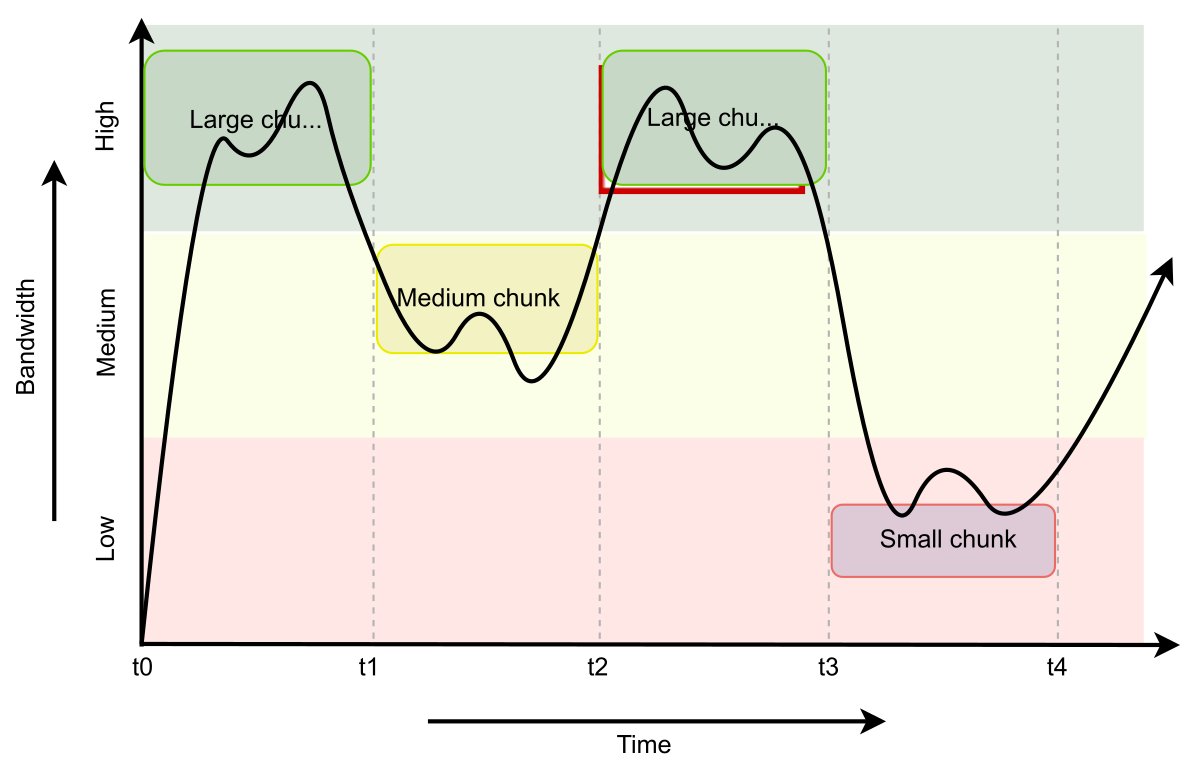
\includegraphics[width=0.5\textwidth]{Images/chapter_26/section_5471711817891840/6680510822875136.png}
 \caption{Chunk size in each time frame provided to the client changes according to the bandwidth}
\end{figure}

The adaptive bitrate algorithm depends on the following four parameters:

\begin{enumerate}
\item
\protect\phantomsection\label{5XOJdpx-sXNmJSO08jqUZ}
End-to-end available bandwidth (from a CDN/servers to a specific client).
\item
\protect\phantomsection\label{RXGpkq03iIODToPSA4_AX}
The device capabilities of the user.
\item
\protect\phantomsection\label{bwVo9FfIYP3Hv7lY58TP3}
Encoding techniques used.
\item
\protect\phantomsection\label{uVklpkb-QDgVcMi3ojk97}
The buffer space at the client {[} source(The Networking Channel: Netflix adaptive streaming and more by Renata and TY){]}.
\end{enumerate}

\begin{figure}[htbp]
 \centering
 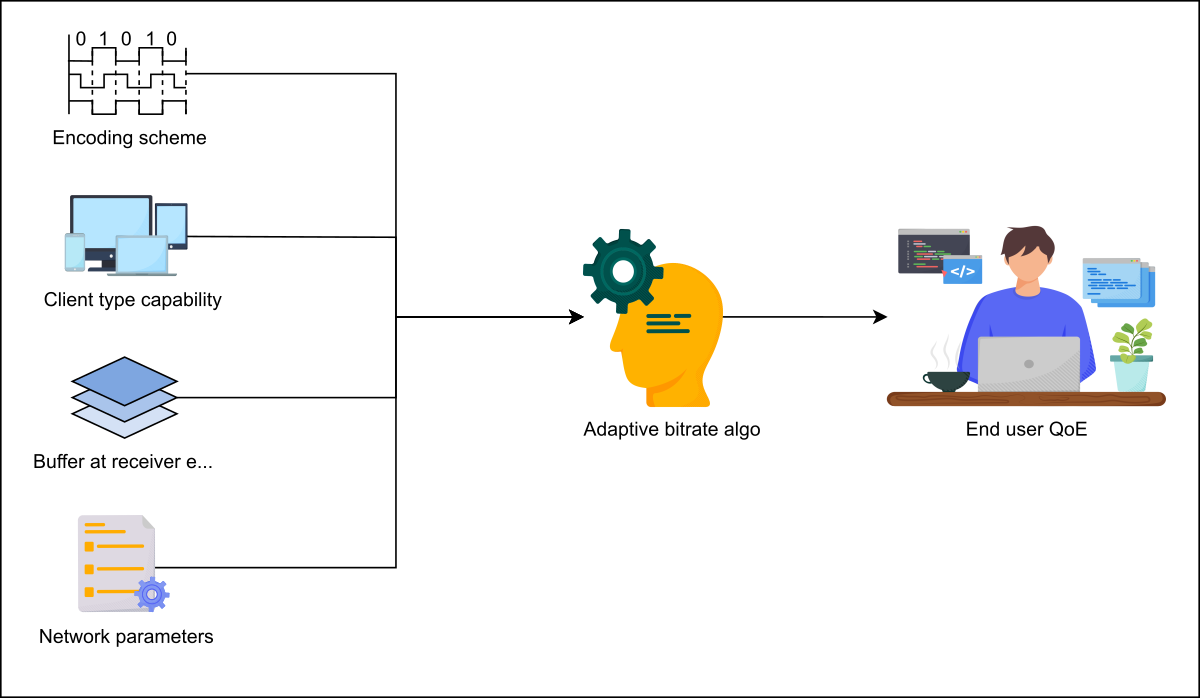
\includegraphics[width=0.5\textwidth]{Images/chapter_26/section_5471711817891840/5071871181979648.png}
 
\end{figure}

We have now discussed the detailed system design of YouTube. In the requirements of YouTube's design, we mentioned the need for our design solution to have low latency as a primary non-functional requirement.
\\
What were the measures taken in our design to ensure low latency?

\textbf{Question:}

State the ways we achieve low latency in the design of YouTube.

\textbf{Reference Answer:}

ISP Cache Servers: Geographically distributed cache servers at the ISP level to keep the most viewed content. Cache : Using caching at various layers via a distributed cache management system. CDNs: Utilizing content delivery networks (CDNs) that make heavy use of caching and mostly serve videos out of memory. A CDN deploys its services in close vicinity to the end users for low-latency services. Video preprocessing: encoding, decoding, and segmentation of the video, different formats for different devices Appropriate storage systems: Choosing appropriate storage systems for different types of data. For example, we can use Bigtable for thumbnails, blob storage for videos, and so on.
\\
Note: The correct answer should have at least 3 of the reasons given above. Explanation is encouraged. Synonyms are allowed.

\subsection{Potential follow-up questions}\label{Kkp5xl3cyt5jnY_yXnDEc}
\\
There can be many different aspects of the system design of YouTube as there is more depth in the subject area. Therefore, many questions can arise. Some questions and directions toward their answers are as follows:

\begin{enumerate}
\item
\protect\phantomsection\label{L7Ys7IjzfcZR_jIn9TqCl}
\textbf{Question}: It is possible to quantify availability by adding numbers like 99.99\% availability or 99.999\% availability. In that case, what design changes will be required? This is a hard question. In reality, such numbers are part of a service's SLA, and they are generated from models or long-term empirical studies. While it is good to know how the above numbers are obtained and how organizations use monitoring to keep availability high, it might be a better strategy to discuss the fault tolerance of the system---what will happen if there are software faults, server failures, full data center failures, and so on. If the system is resilient against faults, that implies the system will have good availability.
\item
\protect\phantomsection\label{it8t2MJOyHH_UE5W7-fyS}
\textbf{Question}: We assumed some reasonable numbers to come up with broad resource requirements. For example, we said the average length of a video is five minutes. In this case, are we designing for average behavior? What will happen to users who don't follow the average profile? A possible answer could be that the above number will likely change over time. Our system design should be horizontally scalable so that with increasing users, the system keeps functioning adequately. Practically, systems might not scale when some aspect of the system increases by an order of magnitude. When some aspects of a system increase by an order of magnitude (for example, 10x), we usually need a new, different design. Cost points of designing 10x and 100x scales are very different.
\item
\protect\phantomsection\label{OWeDKEOsCXolb19RocrO5}
\textbf{Question}: Why didn't we discuss and estimate resources for video comments and likes? Concurrent users' comments on videos are roughly at the same complexity as designing a messaging system. We'll discuss that problem \href{https://www.educative.io/courses/grokking-the-system-design-interview/system-design-whatsapp}{elsewhere} in the course.
\item
\protect\phantomsection\label{gfuokImSTEGj-aY1FB2lZ}
\textbf{Question}: How to manage unexpected spikes in system load? A possible answer is that because our design is horizontally scalable, we can shed some load on the public cloud due to its elasticity features. However, public clouds are not infinitely scalable. They often need a priori business contracts that might put a limit on maximum, concurrently allowed resource use at different data centers.
\item
\protect\phantomsection\label{UPnIbAxyXNSp-ci3NQ6qD}
\textbf{Question}: How will we deploy a global network to connect data centers and CDN sites? In practice, YouTube uses Google's network, which is built for that purpose and peers with many ISPs of the world. It is a fascinating field of study that we have left outside this course for further review.
\item
\protect\phantomsection\label{4Ei_aQxqZvxrfuo_8Q7O1}
\textbf{Question}: Why isn't there more detail on audio/video encoding? There are many audio/video encoding choices, many publicly known and some proprietary. Due to excessive redundancy in multimedia content, encoding is often able to reduce a huge raw format content to a much smaller size (for example, from 600 MB to 30 MB). We have left the details of such encoding algorithms to you if you're interested in further exploration.
\item
\protect\phantomsection\label{1-5h0wLeJCIw2HzO8nULP}
\textbf{Question}: Cant we use specialized hardware (or accelerators like GPUs) to speed up some aspects of the YouTube computation? When we estimated the number of servers, we assumed that any server could fulfill any required functionality. In reality, with the slowing of Moore's law(Moore's law was presented by Gordon Moore in 1965, who stated that the number of transistors in an integrated circuit (IC) doubles every year.), we have special-purpose hardware available (for example, hardware encoders/decoders, machine-learning accelerators like Tensor Processing Units, and many more). All such platforms need their own courses to do justice to the content. So, we avoided that discussion in this design problem.
\item
\protect\phantomsection\label{JzWRqaJErxE56N_vPoTc6}
\textbf{Question}: Should compression be performed at the client-side or the server-side during the content uploading stage? We might use some lossless but fast compression (for example, Google Snappy) on the client end to reduce data that needs to be uploaded. This might mean that we'll need a rich client, or we would have to fall back to plain data if the compressor was unavailable. Both of those options add complexity to the system.
\item
\protect\phantomsection\label{eP-9jmhkXQgwU4r5dPuLG}
\textbf{Question}: Are there any other benefits to making file chunks other than in adaptive bitrates? We discussed video file chunks in the context of adaptive bit rates only. Such chunks also help to parallelize any preprocessing, which is important to meet real-time requirements, especially for live streams. Parallel processing is again a full-fledged topic in itself, and we've left it to you for further exploration.
\end{enumerate}

% End of section content